\section{Introduction}

Real-world distributed programs are challenging to write and maintain
because they inevitably juggle and conflate two distinct mechanisms.
The first concerns the expression of application logic - how do we
define computations that are robust in the presence of distributed
communication among concurrently executing threads of control?  The
second deals with system concerns - how do we express notions of
visibility, replication, and consistency when the nodes participating
in such computations may be geographically distributed and the
networks that connect them unreliable?  To simplify reasoning in such
complicated environments, models often make strong assumptions on the
guarantees provided by an implementation (such as
serializablity~\cite{...} or strong consistency~\cite{...}) that may
inadvertently mask important albeit unpleasant realities related to
network partitions~\cite{...}, or which may ignore important system
architectural features that assume replicated program state~\cite{...}
to provide high availability and fault tolerance.  On the other hand,
when these properties are explicitly exposed to the programmer, e.g.,
by requiring that applications be written in terms of specialized
distributed data structures~\cite{...} or control
primitives~\cite{...}, simplicity, composability, and
ease-of-reasoning suffers.

To illustrate how these kinds of problems manifest in practice,
consider how we might write a simple counter library (see
Fig.~\ref{fig:counter-adt}).  A \C{Counter} supports two (update)
operations - \C{add} and \C{mult} - that lets a non-negative integer
value be added or multiplied to the counter, resp.  Observe that the
library is written in an idiomatic style in OCaml, with no special
reasoning principles needed to realize desired functionality.  As long
as applications use the library on a single machine, this
implementation suffices well.  If the library is used in the context
of a more sophisticated application, say one whose computation is
distributed among a collection of machines, its state may need to be
replicated.  Unfortunately, replication doesn't come for free.  Global
synchronous coordination among all nodes is problematic in distributed
systems.  Thus, applying an \C{Add} operation on one node may not be
instanteously witnessed on another, which may in turn be
simultaneously attempting to perform its own \C{Add} or \C{Mult}
action.  While synchronizing the activities of all nodes to ensure at
most one such operation is performed at a time is impractical,
designating a single node to hold the counter state eschewing
replicating altogether (as in a client-server configuration), is also
an undesirable solution, given its sensitivity to network partitions
and server failures.  But, simply replicating counter state among
nodes, without having any coordination protocol, is an equally
infeasible approach.

A method often adopted~\cite{crdts, pldi15, gotsman-popl16} to address
this tension is to re-define a datatype's operations to return
\emph{effects} instead of values.  An \emph{effect} is a tag that
identifies the operation to be applied uniformly at all replicas to
incorporate the effects of the original
operaton. Fig.~\ref{fig:counter-rdt} shows the \C{Counter} library
with operations re-defined to returns effects.  Observe that the
\C{Counter.add x v} operation now returns an \C{Add x} effect, which,
when applied at a replica (see \C{apply} in the figure), adds \C{x} to
the local counter value.  Assuming effects are commutative, they can
be processed asynchronously using a log local to each replica.  This
implementation produces an eventually consistent global state in which
all replicas will eventually contain the same counter value.  While
effects provide a low-level operational basis for handling replicated
state, the \emph{ad hoc} nature of the solution confounds desirable
high-level reasoning principles.  Indeed, the semantic gap between the
two versions of the counter, one cognizant of replication and the
other not, breaks backward compatibility.  More significantly, its
non-trivial construction must be developed in different guises for
every distributed data structure used by the application.
\begin{figure}
\begin{subfigure}[b]{0.4\textwidth}
  \begin{ocaml}
    module Counter: sig
      type t
      val add: int -> t -> t
      val mult: int -> t -> t
      val read: t -> int
    end = struct
      type t = int
      let add x v = v + (abs x)
      let mult x v = v * (abs x)
      let read v = v
    end
  \end{ocaml}
\caption{\C{Counter} library in OCaml}
\label{fig:counter-adt}
\end{subfigure}
\begin{subfigure}[b]{0.56\textwidth}
  \begin{ocaml}
    module Counter: sig
      type t
      type eff 
      val add: int -> t-> eff
      val mult: int -> t -> eff
      val apply: eff -> t -> t
      val read: t -> int
    end = struct
      type t = int
      type eff = Add of int
      let add x v = Add (abs x)
      let mult x v = Add (v * (abs x - 1))
      let apply (Add x) v = x + v
      let read v = v
    end
  \end{ocaml}
\caption{\C{Counter} library re-engineered for effect-based replication}
\label{fig:counter-rdt}
\end{subfigure}
\end{figure}
Lack of composability is another important downside of this approach.
Consider an application that uses two replicated counters, $c_1$ and
$c_2$, bound by the invariant $c_2 \ge c_1$, duly enforced by the
application when updating $c_2$ or $c_1$.  An execution may
nonetheless witness anamolous states that violate the invariant
because updates to $c_1$ and $c_2$ are applied independently in any
order on any replica.  For example, if a replica increments both
counters, a \C{read} operation performed at another replica may
witness the increment to $c_1$, but not $c_2$, thus violating the
invariant. The intention to atomically apply both effects cannot be
captured in the absence of external mechanisms to compose effects
(such as effect-based transactions~\cite{pldi15}).

On the other hand, a functional programmer is likely to approach the
problems very differently.  Rather than thinking about a low-level
operational variant of distributed state given in terms of explicit
effects as described above, a declarative interpretation of a
decentralized computation could be naturally described in terms of a
version tree whose root contains the initial counter value, and whose
branches represent different versions maintained by different nodes,
with the state produced by a counter's operations on a node recorded
along the node's local branch.  Now, a globally consistent view of a
counter can be explained simply in terms of \emph{merge} operations of
different branch tips.  Treating replication as merging yields a
counter implementation that bears strong similarity to the original
sequential one:
  \begin{ocaml}
    module Counter = struct
      include Counter
      type mergeable_t = t [@@deriving persistence]
      let merge lca v1 v2 = lca + (v1 - lca) + (v2 - lca)
    end
  \end{ocaml}
The role of \C{lca} (least common ancestor) here captures salient
history - the state resulting from the merge of two versions derived
from the same ancestor state should not unwittingly duplicate the
contributions of the ancestor.  This interpretation of a replicated
datatype is thus given in terms of multi-versions of a program state
impicitly associated with the different nodes that comprise a
distributed application and a logical notion of a \emph{master}
representing some consistent, but not necessarily current, view of
global state.
\begin{figure}
  \begin{center}
    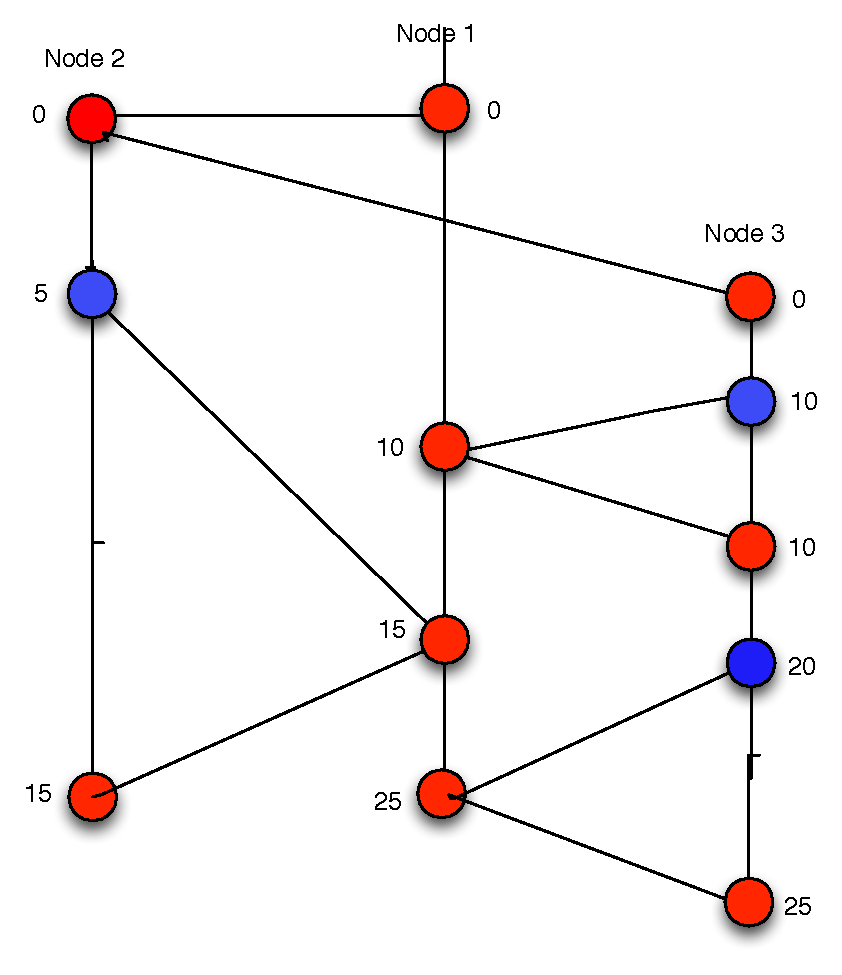
\includegraphics[scale=0.35]{Figures/dali-counter}
  \end{center}
  \caption{\small A multi-version counter can be expressed as a
    sequence of versions managed by logically-distributed concurrently
    executing threads.  Local versions produced by these threads
    periodically merge their state with one another.  In the figure,
    when the local version of Node 3, labeled 20, merges with the
    local version of Node 1, whose counter state is 15 at the time, a
    new counter value is produced.  This value takes into account the
    previous merged state (10) from which the two versions were
    derived to yield a new merged state of 25.  Observe that there is
    no explicit synchronization or coordination among versions.  In
    the figure, red circles represent state produced through merging,
    and blue circles represent local counter state produced by
    applying counter operations on a node-local version.  }
\end{figure}

The \name programming model realizes a monadic functional version
control system centered around data, rather than file coherence.  The
\name monad lets programmers write and compose concurrent computations
around multiple (implicit) versions of a mergeable datatype.  A
computation makes progress by forking concurrent versions of existing
versions, creating later versions along a \emph{branch}, or by merging
branch tips.  An important soundness property of the model is that
instances of a replicated datatype whose merge operation is
commutative with respect to its local version arguments is guaranteed
to eventually converge to the same value on all replicas.  As a
result, OCaml programmers get the benefits of highly available
(low-latency) distributed computation, while continuing to enjoy the
comforts of high-level reasoning and familiarity of standard library
datatypes.  Notably, while \name's programming model makes no explitic
reference to any specific operational manifestation of a distributed
system (e.g., programmers do not need to worry about replicas and
their management), it can be nonetheless efficiently realized on
existing geo-replicated distributed systems.

Our contributions are summarized below:

\begin{itemize}
    \item We formally introduce the concept of a \emph{mergeable} datatype
      to admit high-level declarative reasoning about distributed
      computation and replicated state in functional programs.

    \item We describe the \name library that transparently adds
      persistence and replication features to a mergeable type. \name
      comes with a programming model that brings to bear the power and
      flexibility of a version control system to the administration of
      replicated data. \name hides the complexity of version control
      behind a monad, and exposes its functionality via a simple API
      that lets programmers define and compose concurrent OCaml
      computations around such data.  Issues related to replication
      only manifest implicitly in the definition of a merge operation
      that defines coherence among different instances of replicated
      state.

    \item We present a formalization of the \name programming model,
      and establish the comditions under which eventual convergence of
      concurrent version state can be guaranteed.

    \item We describe an implementation of \name atop the Irmin
      persistent store~\cite{...}, a content-addressable storage
      library for OCaml, along with case studies and experimental
      results to its practical utility.
\end{itemize}



%% Persistence adds yet another dimension to the problem. Functional data
%% structures are often large in-memory linked structures that admit
%% functional updates by creating newer versions that share most of their
%% structure with previous versions. Sharing is the key to efficiency,
%% without which every functional update takes time that is at least
%% linear in the size of the data structure. Unfortunately, the
%% straightforward way to persist a data structure on disk in a
%% machine-agnostic format (e.g., JSON) requires serialization, which is
%% linear in the size of the data structure. An alternative is to
%% maintain a separate on-disk copy of the data and administer it via a
%% database system. The downside is that the programmer is now required
%% to reason in terms of a lower-level abstraction (e.g., a relational
%% data model) in order to maintain coherence between in-memory and
%% on-disk representations. Safety guarantees over the in-memory data do
%% not carry over to the disk, which introduces additional complications
%% and the possibility of new bugs. Thus, adding persistence to
%% applications while preserving high-level safety gurantees offered by
%% the language abstraction is a non-trivial problem.



%% However, as we shall see,
%% unconstrained branching may yield a branching structure that becomes
%% unmergeable, thus leading to \emph{stuck} states. An important
%% property of the \name library is that it guarantees progress even in
%% the presence of arbitrary merges provided the merge operation is
%% commutative with respect to its version state arguments.  Furthermore,
%% \name profitably exploits provenance information available via
%% branches to make application resilient to network partitions.  
%% In this paper, we define a semantics of mergeable datatypes that lets
%% any OCaml program be seamlessly deployed in a distributed environment
%% with implicit support for replicated and decentralized operation.  The
%% underlying foundation for merge actions has a natural category
%% theoretic interpretation that enables us to construct useful mergeable
%% variants for \emph{any} OCaml type whose states are commutative wtih
%% respect to the merge operation defie
